\chapter{ГЛАВА НОМЕР ДВА --- СОДЕРЖАТЕЛЬНАЯ}
\label{ch:2}
    \section{Работаем с текстом}
        \subsection{Жирный, курсив}
        А вообще, текст может быть разным \textbf{ЖИИИРНЫМ} или \textit{КУУУУРСИВНЫМ}.
        \subsection{Цитирование}
        Ещё можно цитировать вот так\cite{bellman2003dynamic, gartner_definition, FRS1901LIIIOL}.
        Стоит отметить, что раздел <<список использованных источников>> формируется автоматически из файла <<biba.bib>>. Чтобы цитировать статью или книгу не нужно вручную вбивать все поля, достаточно найти эту статью, например, на <<researchgate>>, нажать на кнопку <<\href{https://www.researchgate.net/publication/346702745_Cooperative-Coevolution-CMA-ES_with_Two-Stage_Grouping/citation/download}{download citation}>> , выбрать <<BibTeX>> и вставить в файлик для цитирований. В списке он появится только тогда, когда вы впервые процитируете этот источник в тексте\cite{inproceedings}.
    
    
     
    \section{Делаем таблички}
        \begin{tabular}{l||l|cc}
            \hline
            № & ФИО & Возраст & Стаж (лет)\\
            \hline\hline
            1 & Иванов П.М. & 45 & 17 \\
            2 & Петров Д.А. & 56 & 28 \\
            3 & Егоров K.А. & 48 & 21
        \end{tabular}


    \section{Списки}
        Перечислим что-нибудь
        \begin{itemize}
            \item Один
            \item Два
            \item Три
            \item Четыре
        \end{itemize}


    \section{Формулы}
        \begin{gather}
            lb_i \leq X_i \leq ub_i,\   i = \overline{1, 940}.\label{eq:1}
        \end{gather}

        \begin{gather}
            \arraycolsep=1.4pt\def\arraystretch{1.8}
            \boldsymbol{Minimize}\ f = \left ( \sum_{i=1}^{N_1} {{Rem_A}_{(i)}} + \sum_{i=1}^{N_1} {Rem_B}_{(i)}\right) + C_{DSO} \cdot F_{match};\label{eq:2}\\
            {Rem_A}_{(i)} =   \begin{cases}
                {C_A}_{(i)},  & \mbox{if } t_{start(i)} \neq t_{new(i)} \\
                0, & \mbox{otherwise}
                            \end{cases};\label{eq:3}\\
            Rem_{B_{(i)}} = C_{B(i)} \cdot \sum_{i=1}^{N_T} \mid B_{base(j, t)} - B_{flex(j, t)} \mid ; \label{eq:4} \\
            F_{match} = \sum_{i=1}^{N_T} \mid F_{agg(t)} - F_{DSO(t)}\mid ; \label{eq:5} 
        \end{gather}


        $
        \begin{cases}
        a_{13}' = a_{11} x_0 + a_{12} y_0 + a_{13} = 0\\
        a_{23}' = a_{12} x_0 + a_{22}y_0 + a_{23} = 0
        \end{cases} \Longleftrightarrow
        \begin{pmatrix}
        5 & 6 \\
        6 & 0 
        \end{pmatrix} \cdot \begin{pmatrix}
        x_0 \\ 
        y_0
        \end{pmatrix} = 
        \begin{pmatrix}
        11 \\ 
        6
        \end{pmatrix}
        $

    \section{Псевдокод}
        \begin{algorithm}
            \caption{CBCC-RDG3}\label{alg:CBCC-RDG3}
            \begin{algorithmic}[1]
            \State divide decision parameters X into subsets $X_i$: $1 <= i <= m$, using RDG3
            \State $x^{*}$ - a context vector
            \For{$i$ from 1 to $iter_{max}$}
            \For{$i$ from 1 to $m$ }
            \State Find optimal solution for the sub-component using CMA-ES
            \State Update $x^{*}$
            \EndFor
            \EndFor
            \State return $x*$
            \end{algorithmic}
        \end{algorithm}

    \newpage
    \section{Графика и картинки}

    Одну схему/график/картинку можно вставить так
    \begin{figure}[ht!]
    \center{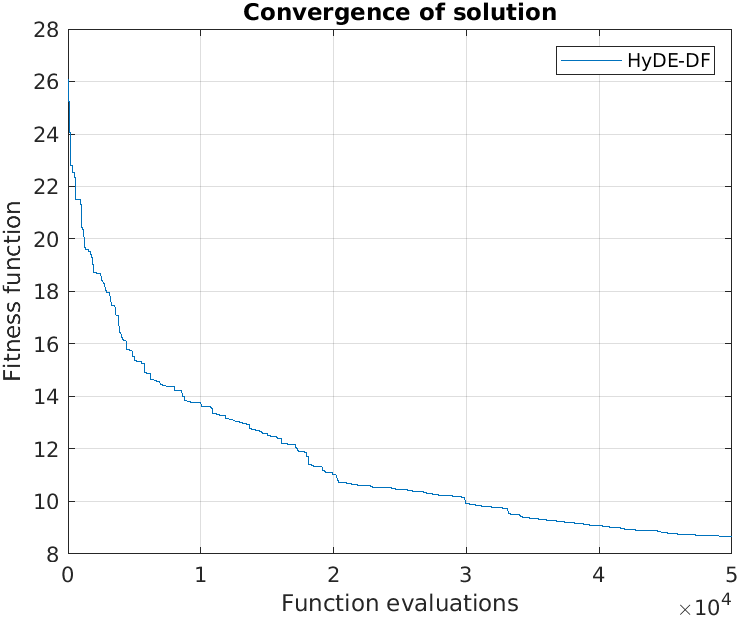
\includegraphics[width=0.5 \textwidth]{images/Examples/HyDE_50000.png}}
    \caption{\label{fig:Model_of_Edge} Вставка одного графика }
    \end{figure}

    Два графика на одном уровне
    \begin{figure}[ht!]
        \centering
        \begin{subfigure}{.5\textwidth}
          \centering
          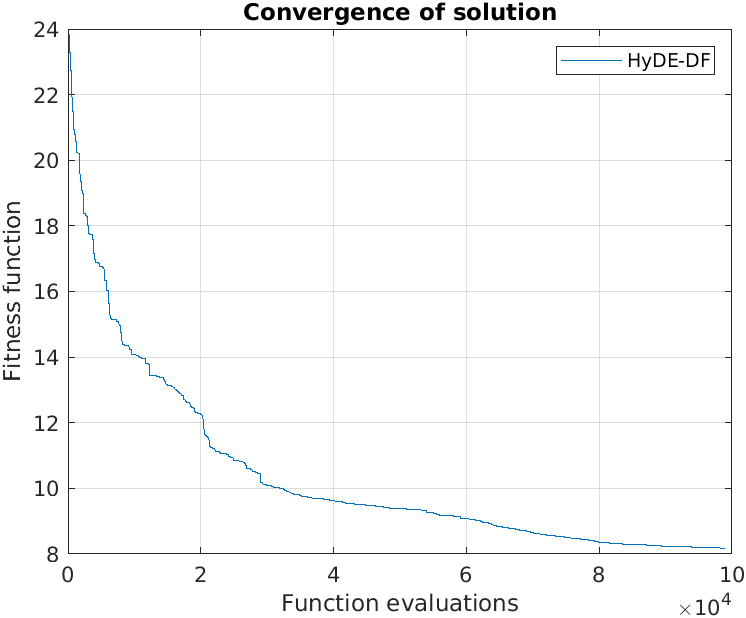
\includegraphics[width=.9\linewidth]{images/Examples/HyDE_100000.png}
          \caption{Левый график}
          \label{fig:sub1}
        \end{subfigure}%
        \begin{subfigure}{.5\textwidth}
          \centering
          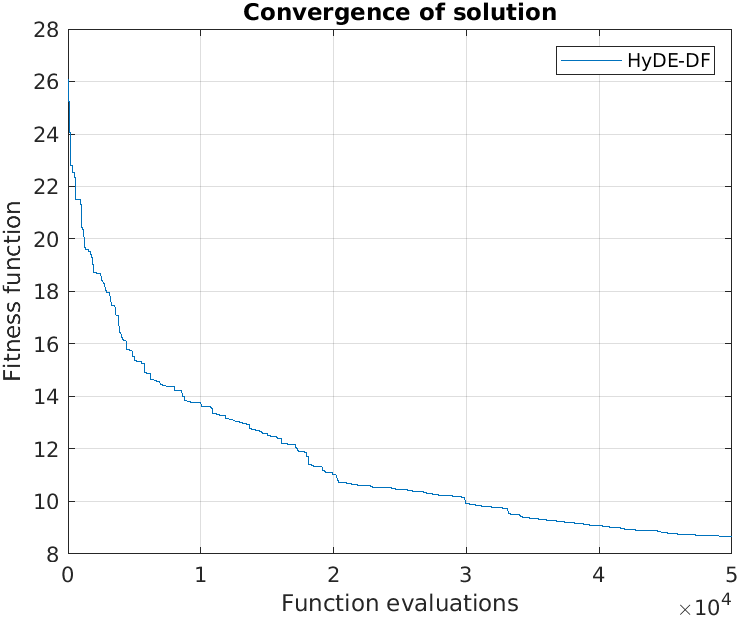
\includegraphics[width=.9\linewidth]{images/Examples/HyDE_50000.png}
          \caption{Правый график}
          \label{fig:sub2}
        \end{subfigure}
        \caption{Вставка двух графиков на одном уровне}
        \label{fig:test}
    \end{figure}
